%
% This is the LaTeX template file for lecture notes for EE 382V.
%

\documentclass[twoside]{article}
\usepackage{graphicx}
\graphicspath{ {images/} }
\setlength{\oddsidemargin}{0.25 in}
\setlength{\evensidemargin}{-0.25 in}
\setlength{\topmargin}{-0.6 in}
\setlength{\textwidth}{6.5 in}
\setlength{\textheight}{8.5 in}
\setlength{\headsep}{0.75 in}
\setlength{\parindent}{0 in}
\setlength{\parskip}{0.1 in}

%
% The following commands set up the lecnum (lecture number)
% counter and make various numbering schemes work relative
% to the lecture number.
%
\newcounter{lecnum}
\renewcommand{\thepage}{\thelecnum-\arabic{page}}
\renewcommand{\thesection}{\thelecnum.\arabic{section}}
\renewcommand{\theequation}{\thelecnum.\arabic{equation}}
\renewcommand{\thefigure}{\thelecnum.\arabic{figure}}
\renewcommand{\thetable}{\thelecnum.\arabic{table}}

%
% The following macro is used to generate the header.
%
\newcommand{\lecture}[4]{
   \pagestyle{myheadings}
   \thispagestyle{plain}
   \newpage
   \setcounter{lecnum}{#1}
   \setcounter{page}{1}
   \noindent
   \begin{center}
   \framebox{
      \vbox{\vspace{2mm}
    \hbox to 6.28in { {\bf EE 382V: Social Computing
                        \hfill Fall 2018} }
       \vspace{4mm}
       \hbox to 6.28in { {\Large \hfill Lecture #1: #2  \hfill} }
       \vspace{2mm}
       \hbox to 6.28in { {\it Lecturer: #3 \hfill Scribe: #4} }
      \vspace{2mm}}
   }
   \end{center}
   \markboth{Lecture #1: #2}{Lecture #1: #2}
   %{\bf Disclaimer}: {\it These notes have not been subjected to the
   %usual scrutiny reserved for formal publications.  They may be distributed
   %outside this class only with the permission of the Instructor.}
   \vspace*{4mm}
}

%
% Convention for citations is authors' initials followed by the year.
% For example, to cite a paper by Leighton and Maggs you would type
% \cite{LM89}, and to cite a paper by Strassen you would type \cite{S69}.
% (To avoid bibliography problems, for now we redefine the \cite command.)
% Also commands that create a suitable format for the reference list.
\renewcommand{\cite}[1]{[#1]}
\def\beginrefs{\begin{list}%
        {[\arabic{equation}]}{\usecounter{equation}
         \setlength{\leftmargin}{2.0truecm}\setlength{\labelsep}{0.4truecm}%
         \setlength{\labelwidth}{1.6truecm}}}
\def\endrefs{\end{list}}
\def\bibentry#1{\item[\hbox{[#1]}]}

%Use this command for a figure; it puts a figure in wherever you want it.
%usage: \fig{NUMBER}{SPACE-IN-INCHES}{CAPTION}
\newcommand{\fig}[3]{
			\vspace{#2}
			\begin{center}
			Figure \thelecnum.#1:~#3
			\end{center}
	}
% Use these for theorems, lemmas, proofs, etc.
\newtheorem{theorem}{Theorem}[lecnum]
\newtheorem{lemma}[theorem]{Lemma}
\newtheorem{proposition}[theorem]{Proposition}
\newtheorem{claim}[theorem]{Claim}
\newtheorem{corollary}[theorem]{Corollary}
\newtheorem{definition}[theorem]{Definition}
\newenvironment{proof}{{\bf Proof:}}{\hfill\rule{2mm}{2mm}}

% **** IF YOU WANT TO DEFINE ADDITIONAL MACROS FOR YOURSELF, PUT THEM HERE:

\begin{document}
%FILL IN THE RIGHT INFO.
%\lecture{**LECTURE-NUMBER**}{**DATE**}{**LECTURER**}{**SCRIBE**}
\lecture{3 Session 1}{September 28}{Vijay Garg}{Bhargavi Karthik}

\section{LP-Duality}
In Kuhn-Munkres (KM) algorithm, we find matching using the concept of labeling the vertices such that it satisfies the feasibility constraints. Using LP-Duality, we can come up with similar ideas for solving problems in a more intuitive way.

\subsection{Example for LP Duality}
There is an objective function which we are trying to minimize,

 \hspace{10mm} 7$x_1$ + $x_2$ + 5$x_3$ 
 
subject to constraints,
 
 \hspace{10mm} $x_1$ - $x_2$ + 3$x_3$ $\geq$ 10
 
 \hspace{10mm} 5$x_1$ + 2$x_2$ - $x_3$ $\geq$ 6
 
where $x_1$, $x_2$, $x_3$ are the decision variables and assumption is that,

 \hspace{10mm} $x_1$, $x_2$, $x_3$ $\geq$ 0

\begin{figure}[h]
    \centering
    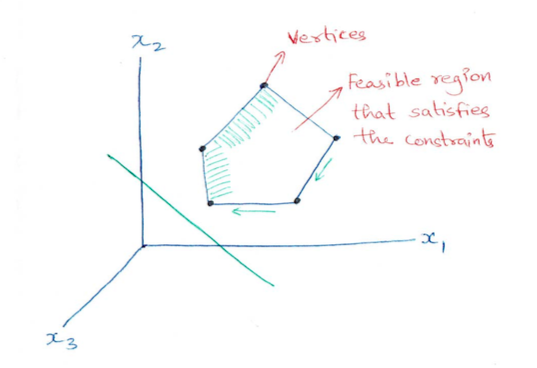
\includegraphics[width=0.6\textwidth]{LP-Duality.png}
    \caption{Finding optimal solution in the feasible space}
    \label{fig:lp1}
\end{figure}

Every constraint is in some sense dividing up the feasible region into two half spaces. The goal here is to find the optimal solution. If we can draw level sets for the given objective function, which means we are trying to optimize along some dimension. In this case we are trying to find the minimum. While trying to optimize along some direction, the point one always hits will be a corner. One of the important properties as per the Simplex algorithm is - "The extremal point is always a vertex". 

The approach is to figure out one feasible point and start from there. If it is not a corner, keep moving until we find a corner and keep optimizing. However, if we are at a corner and if there are n other corners to go to, then go in the direction that has the most advantage.

Suppose we have solution, x = (2, 1, 3). Lets substitute in the objective function,

\hspace{10mm} 7(2) + 1 + 5(3) = 14 + 1 + 15 = 30

this solution is also feasible as it satisfies the constraints,

\hspace{10mm} 2 - 1 + 3(3) = 10 

\hspace{10mm} 5(2) + 2(1) - 3 = 9

Trying to find a bound on primal:

\hspace{10mm} 7$x_1$ + $x_2$ + 5$x_3$ $\geq$ $x_1$ - $x_2$ + 3$x_3$ $\geq$ 10
by comparing coefficients point-wise and $x_i$ $\geq$ 0

solution has to be $\geq$ 10 but we are trying to get a better or greater lower bound

Add up the constraints equations,

\hspace{10mm} 6$x_1$ + $x_2$ + 2$x_3$ $\geq$ 16

The objective function is still greater than the above equation. Hence new lower bound is 16.
\begin{figure}[h]
    \centering
    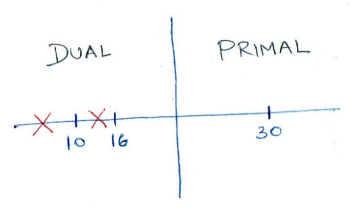
\includegraphics[width=0.4\textwidth]{Primal-Dual.png}
    \caption{Representation of the example as duality}
    \label{fig:lp2}
\end{figure}

The goal of primal was to minimize and so now the goal of dual will be to maximize. We have to figure out what combination of each constraint should we add such that it gives the tightest bound on the objective function.

We have n decision variables and m constraints in our primal. So dual will have m variables (one variable for each constraint in primal) and n constraints (since n decision variables in primal).

Objective function is 10$y_1$ + 6$y_2$ subject to constraints,

\hspace{10mm} $y_1$ + 5$y_2$ $\leq$ 7

\hspace{10mm} -$y_1$ + 2$y_2$ $\leq$ 1

\hspace{10mm} 3$y_1$ - $y_2$ $\leq$ 5

In a generalized representation of the primal, objective function can be written as 
$$\sum_{i=1}^{n} c_i x_i$$
constraints can be written as $$ \sum_{j}^{} {A_i}_j x_j \geq b_j $$
where A is a matrix of dimension m*n, c and b are vectors of size n and m respectively. 

For dual, b is translated to c, c is translated to b and matrix A becomes $A^T$.

\subsection{Strong Duality}
\begin{theorem}
The primal program has finite optimum if and only if its dual has finite optimum. Moreover, if $x*$ and $y*$ are optimal solutions for (P) and (D) then,
$$\sum_{j=1}^{n} c_j x_j^* = \sum_{i=1}^{m} b_i y_i^*$$
\end{theorem}
Note: This translates into all the min-max theorems such as max flow = min cut, max matching = min vertex cover and min number of chains to cover a poset = max sized anti-chain

\subsection{Weak Duality}
\begin{theorem}
If x and y are feasible solutions for (P) and (D) then,
$$\sum_{j=1}^{n} c_j x_j \geq \sum_{i=1}^{m} b_i y_i$$
\end{theorem}
\begin{proof}
\begin{claim}
\label{wdtc1}
$$\sum_{j=1}^{n} c_j x_j \geq \sum_{j=1}^{n} (\sum_{i=1}^{m} {a_i}_j y_i) x_j$$
This claim is true because y is feasible and $x \geq 0$
\end{claim}
\begin{claim}
\label{wdtc2}
$$\sum_{i=1}^{m} (\sum_{j=1}^{n} {a_i}_j x_j) y_i \geq \sum_{i=1}^{m} b_i y_i$$
This claim is true because x is feasible and $y \geq 0$
\end{claim}
Equating claim \ref{wdtc1} to claim \ref{wdtc2}

Hence proved, $$\sum_{j=1}^{n} c_j x_j \geq \sum_{i=1}^{m} b_i y_i$$
\end{proof}

\subsection{Complementary Slackness Conditions}
\begin{theorem}
Given that x,y are (P) and (D) feasible solutions. Then x and y are both optimal if and only if the following complementary slackness conditions are satisfied:
\begin{claim}
$$\forall j \quad either (x_j=0) \quad or \quad \sum_{i=1}^{m} {a_i}_j y_i = c_j$$
\end{claim}
\begin{claim}
$$\forall i \quad either (y_i=0) \quad or \quad \sum_{j=1}^{n} {a_i}_j x_j = b_i$$
\end{claim}
\end{theorem}

\section{LP Duality and Maximum Matching}
For the Kuhn-Munkres Algorithm, we started with x variables and came up with labels through initial feasible labeling. These labels are the dual variables. And we tried to get complementary slackness.

\subsection{Maximum Matching Problem As Linear Program}
\textbf{Primal:}
$$max \sum_{i,j}^{} {W_i}_j {x_i}_j$$
subject to:
$$\sum_{j}^{} {x_i}_j \leq 1$$ and $$\sum_{i}^{} {x_i}_j \leq 1$$
where ${x_i}_j$ is an edge between A and B, i is an index from A and j is an index from B. For each edge, there is a weight ${W_i}_j$. We need to pick the edges such that the sum of their weights is maximum.

Replacing integral constraint by linear constraint,
$${x_i}_j \in \big\{0, 1\big\} \Rightarrow {x_i}_j \geq 0$$
The above transformation is called LP-Relaxation. This can be used only when we can prove that the optimal solution is always going to be integral.

When $|A| = |B| = n$

Number of decision variables = $n^2$

Number of constraints = 2n

\textbf{Dual:}

Number of decision variables = 2n

Number of constraints = $n^2$

Objective function (minimizing vertex labels): $$min \sum_{}^{} u_i + \sum_{}^{} v_j$$

subject to: 
$u_i + v_j \geq {w_i}_j$

$u_i \geq 0 \quad and \quad v_j \geq 0$

where $u_i$ is constraints for side A and $v_j$ is constraints for side B
\end{document}